\pagestyle{fancy}
\part{Momento centrifugo}
\setcounter{section}{0}
\section{La definizione di momento centrifugo}
%--------------------------------------------------------------------------------------------------------------------------------------------------------------
\renewcommand{\thefigure}{3~-~1}
\begin{figure}[ht]
\centering
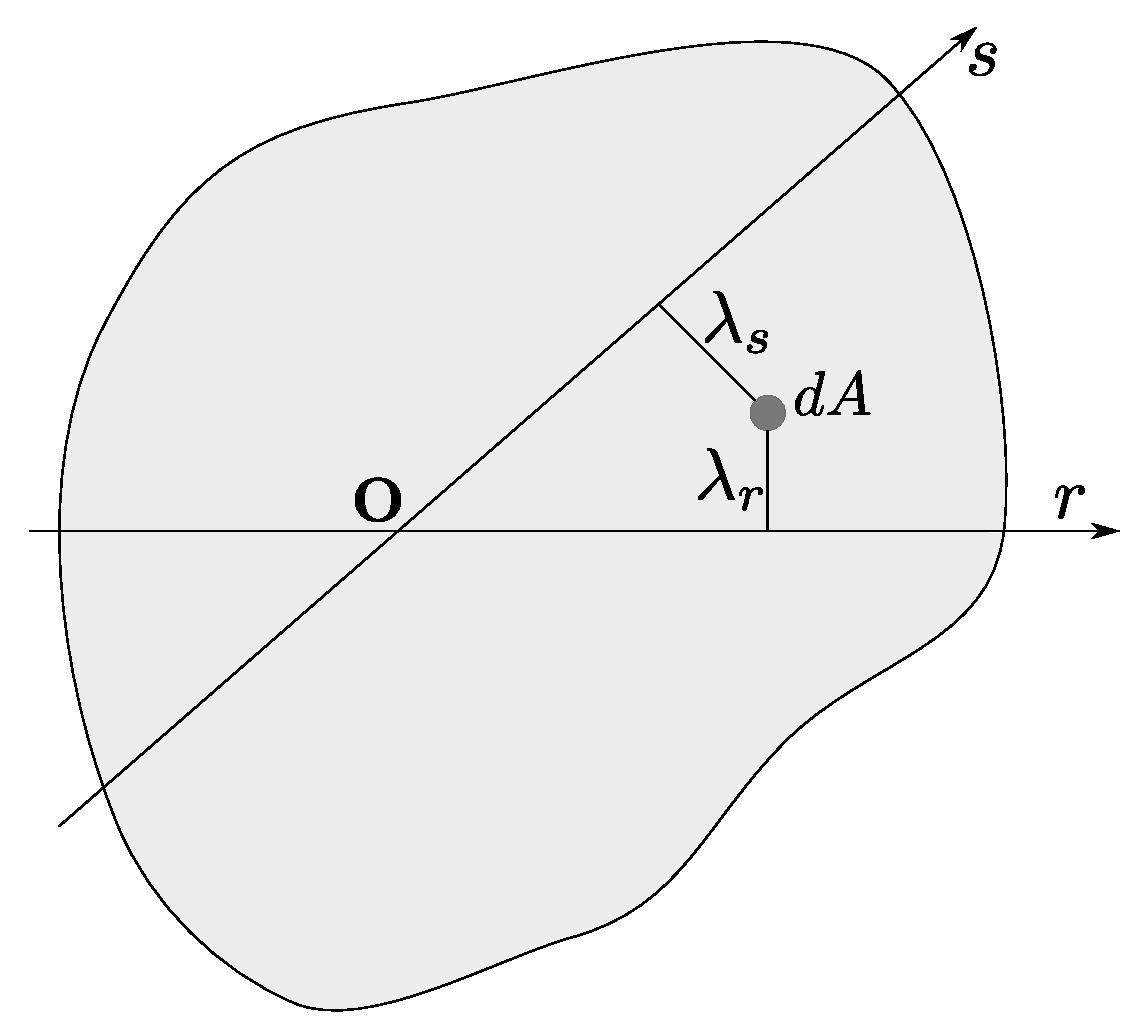
\includegraphics[width=0.55\textwidth]{Immagini/Parte_3/Figura3_1/Figura3_1.pdf}
\caption{}
\label{figura3-1}
\end{figure}
%--------------------------------------------------------------------------------------------------------------------------------------------------------------
Con riferimento alla figura~\ref{figura3-1} si dice momento centrifugo della figura piana rispetto alle rette \textsc{orientate} $r$ ed $s$ la quantità
%--------------------------------------------------------------------------------------------------------------------------------------------------------------
\begin{equation} \label{equazione3-1}
\boxed{I_{rs}=\int\int_A \lambda_{r}\lambda_{s}dA} \tag{3.1}
\end{equation}
%--------------------------------------------------------------------------------------------------------------------------------------------------------------
È evidente che può essere $I_{rs}$ maggiore o minore di zero e che le sue dimensioni fisiche sono $[L^4]$. Rispetto agli assi cartesiani il momento centrifugo si esprime, ovviamente, come
%--------------------------------------------------------------------------------------------------------------------------------------------------------------
\begin{equation} \label{equazione3-2}
\boxed{I_{xy}=\int\int_A xydA} \tag{3.2}
\end{equation}
%--------------------------------------------------------------------------------------------------------------------------------------------------------------
Si potrebbe dimostrare la seguente proposizione
%--------------------------------------------------------------------------------------------------------------------------------------------------------------
\newcommand{\parallelsum}{\mathbin{\!/\mkern-5mu/\!}}
\begin{equation*}
\boxed{\textup{\small Se $r_0$ è un asse di simmetria, ortogonale o no, rispetto alla direzione}\,\delta\textup{\small, risulta:}\,\,I_{r_{0}s}=0\,\,\forall s\parallelsum\delta}
\end{equation*}
%%--------------------------------------------------------------------------------------------------------------------------------------------------------------
\renewcommand{\thefigure}{3~-~2}
\begin{figure}[ht]
\centering
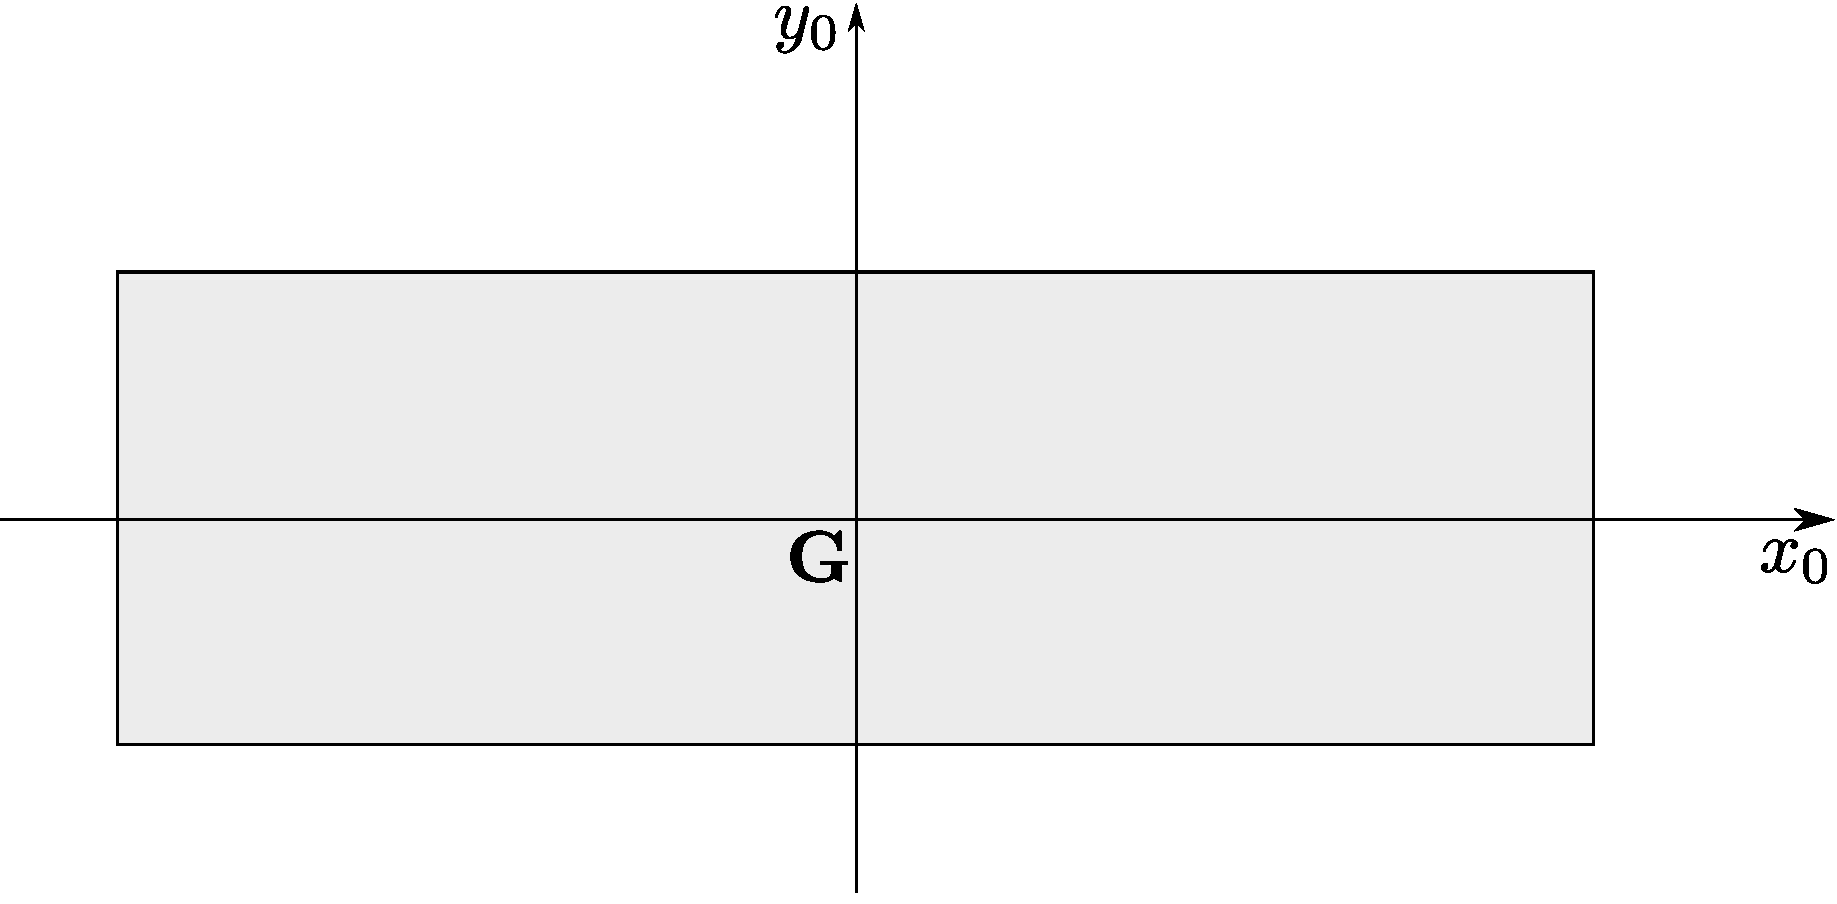
\includegraphics[width=0.37\textwidth]{Immagini/Parte_3/Figura3_2/Figura3_2.pdf}
\caption{$I_{xy_{0}} = 0 \quad \forall\,x\,\parallelsum\,x_0$   ;   $I_{x_{0}y} = 0 \quad \forall\,y\,\parallelsum\,y_0$}
\label{figura3-2}
\end{figure}
%--------------------------------------------------------------------------------------------------------------------------------------------------------------
\renewcommand{\thefigure}{3~-~3}
\begin{figure}[h]
\centering
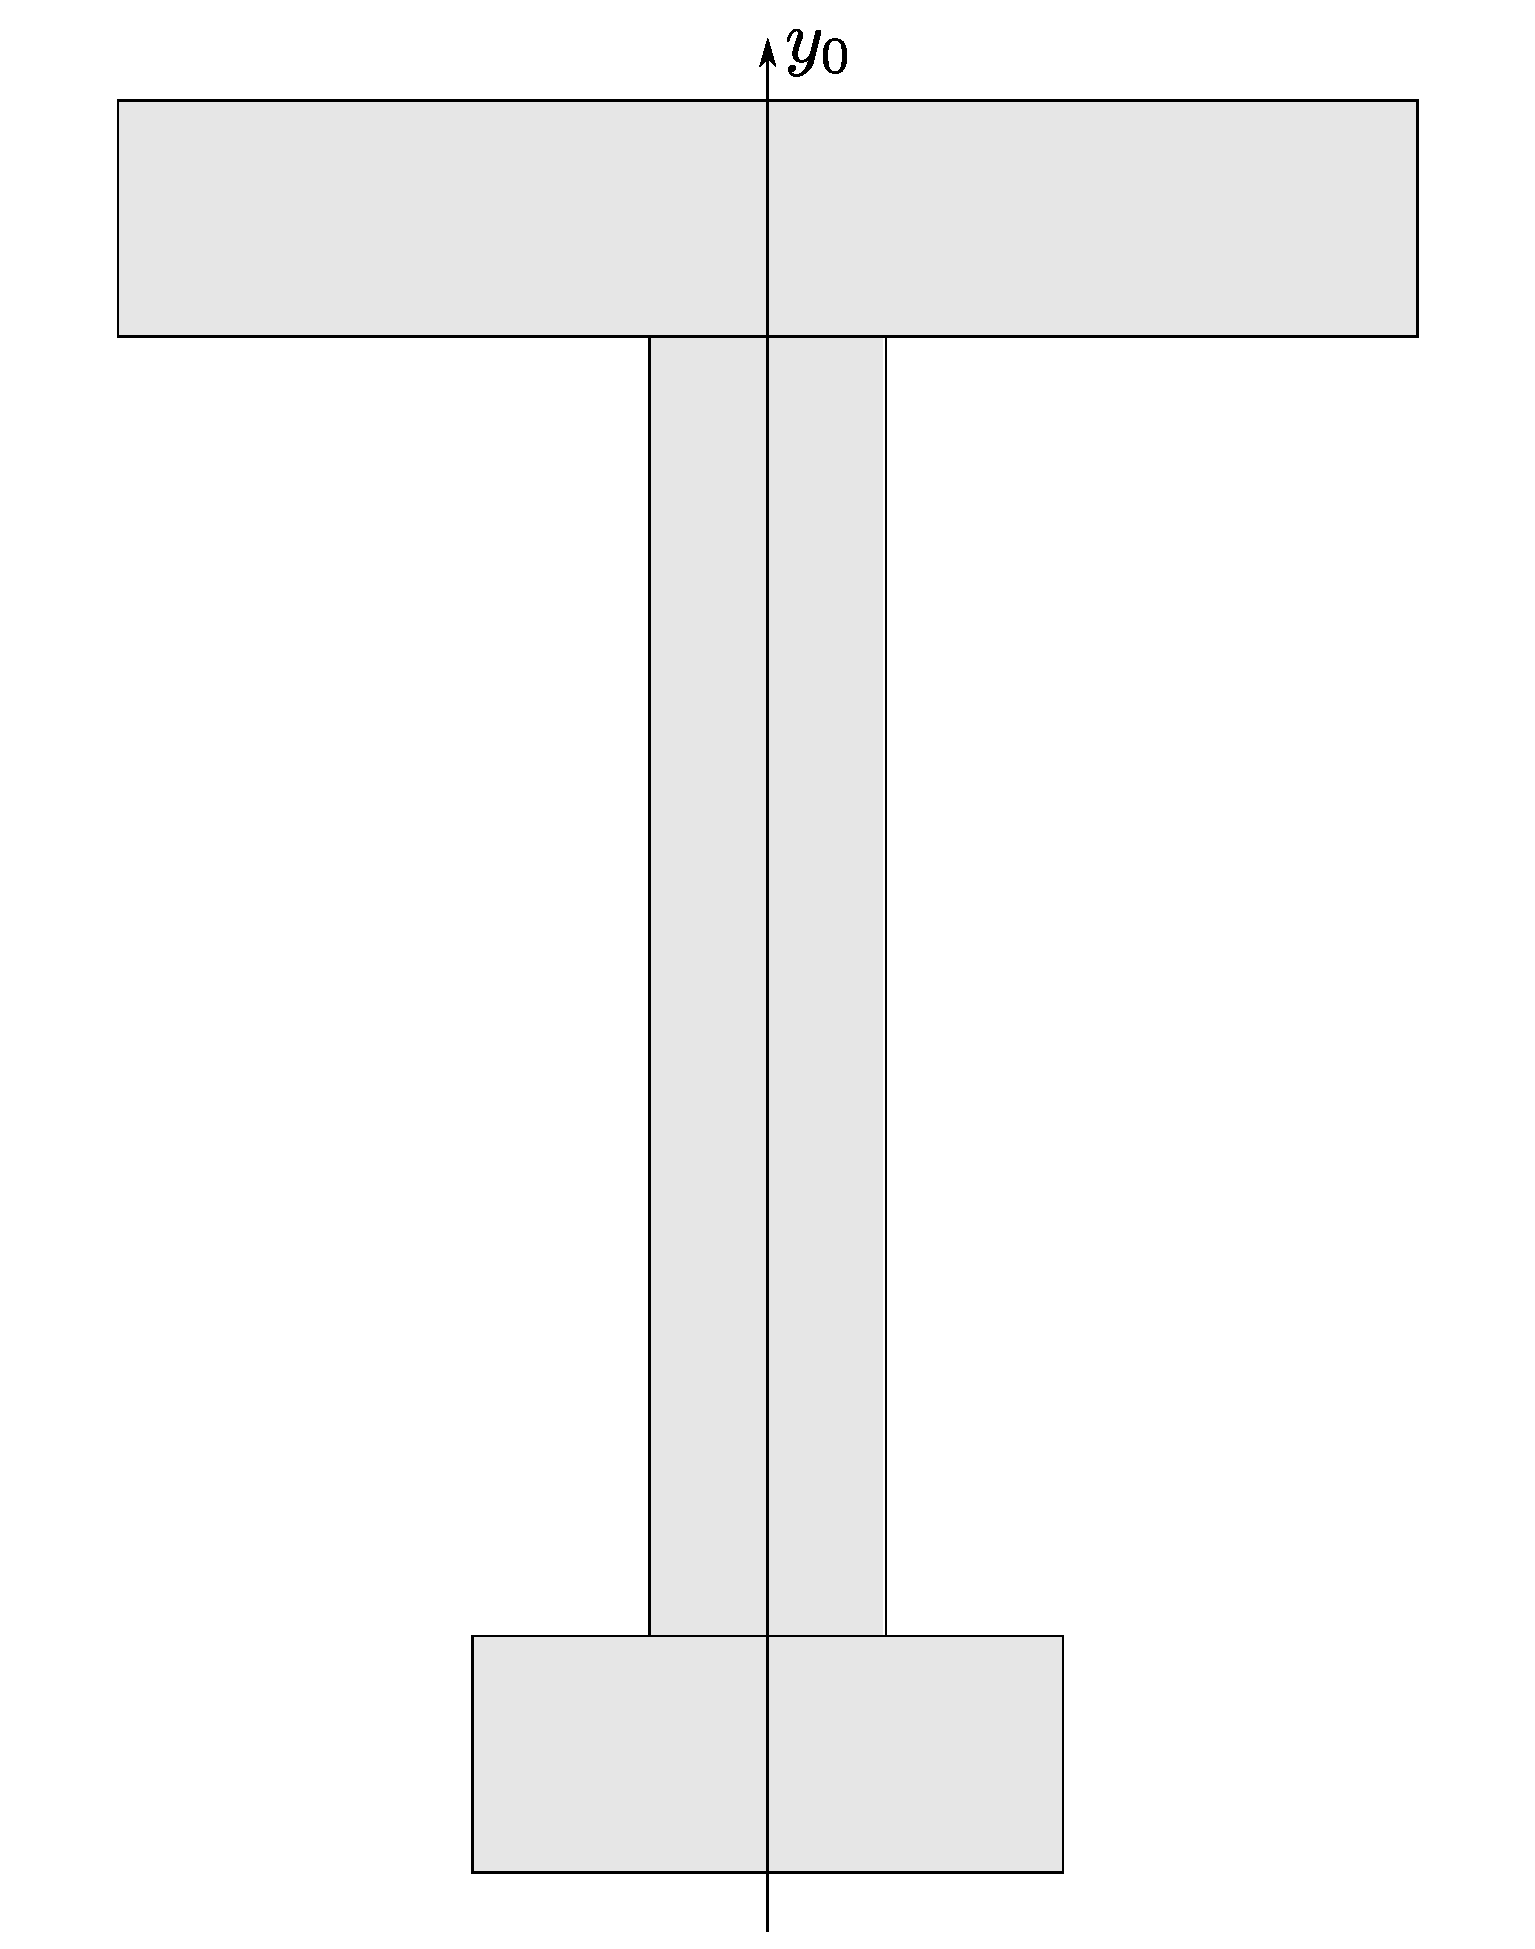
\includegraphics[width=0.34\textwidth]{Immagini/Parte_3/Figura3_3/Figura3_3.pdf}
\caption{$I_{xy_{0}} = 0 \quad \forall\,x\,\bot\,x_0$}
\label{figura3-3}
\end{figure}
%--------------------------------------------------------------------------------------------------------------------------------------------------------------
\renewcommand{\thefigure}{3~-~4}
\begin{figure}[h!]
\centering
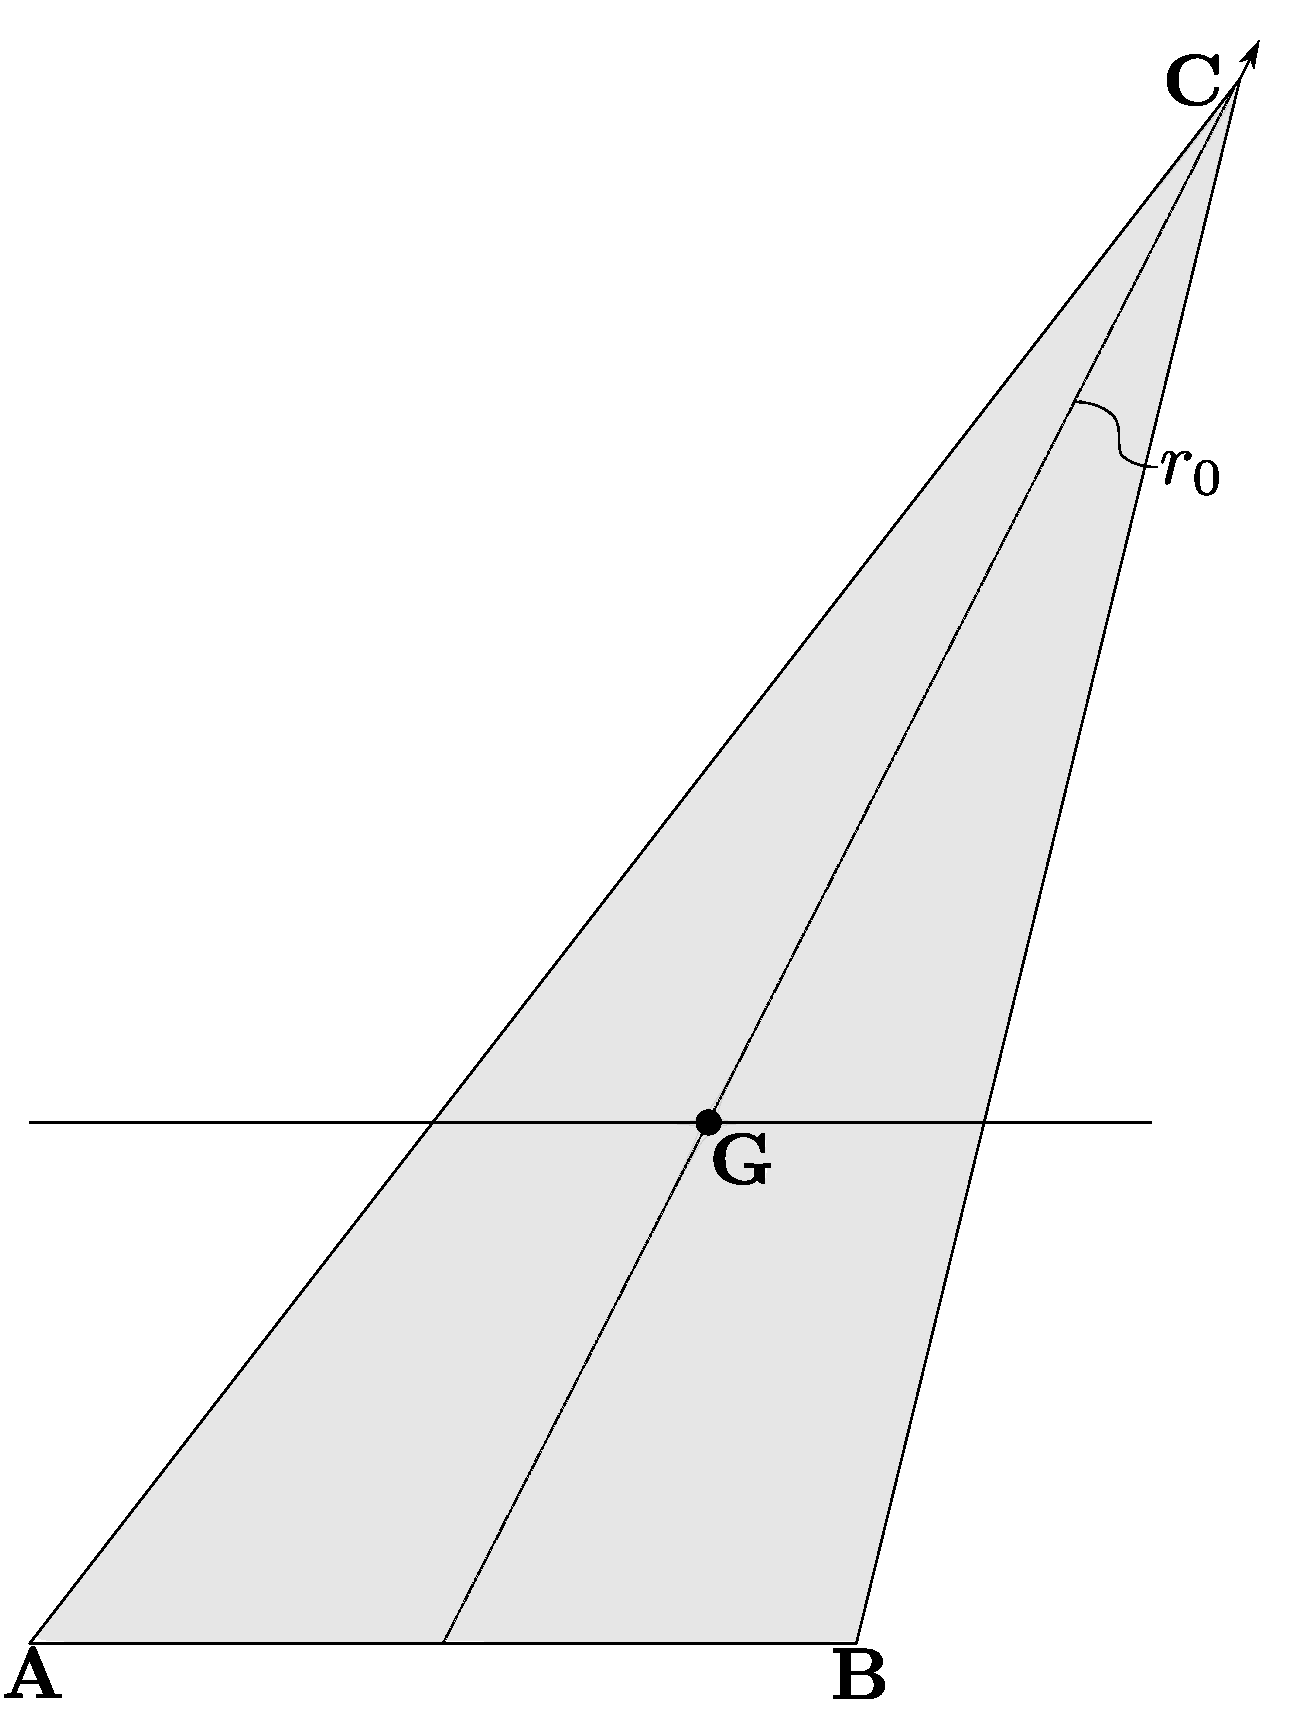
\includegraphics[width=0.34\textwidth]{Immagini/Parte_3/Figura3_4/Figura3_4.pdf}
\caption{$I_{r_{0}s} = 0 \quad \forall\,x\,\parallelsum\,AB$}
\label{figura3-4}
\end{figure}
%--------------------------------------------------------------------------------------------------------------------------------------------------------------
%--------------------------------------------------------------------------------------------------------------------------------------------------------------

\noindent Le figure~\ref{figura3-2},~\ref{figura3-3} e~\ref{figura3-4} illustrano la suddetta proposizione.
%--------------------------------------------------------------------------------------------------------------------------------------------------------------

\noindent Semplicemente osservando la~\eqref{equazione3-1} ci si rende conto, infine, della validità delle seguenti proposizioni
%--------------------------------------------------------------------------------------------------------------------------------------------------------------
\begin{equation*}
\boxed{\textup{\small Se si scambia verso ad uno dei due assi del riferimento, il momento centrifugo cambia segno}}
\end{equation*}
\begin{equation*}
\boxed{\textup{Se si cambia verso ad entrambi il momento centrifugo resta invariato}}
\end{equation*}
%--------------------------------------------------------------------------------------------------------------------------------------------------------------
In simboli
%--------------------------------------------------------------------------------------------------------------------------------------------------------------
\begin{align}
I_{(-r)s}    &= -I_{rs} \tag{3.3a} \label{equazione3-3a} \\ 
I_{r(-s)}    &= -I_{rs} \tag{3.3b} \label{equazione3-3b}\\ 
I_{(-r)(-s)} &= I_{rs} \tag{3.3c} \label{equazione3-3c}
\end{align}
%--------------------------------------------------------------------------------------------------------------------------------------------------------------
\section{Teorema del trasporto del momento centrifugo}
%--------------------------------------------------------------------------------------------------------------------------------------------------------------
\renewcommand{\thefigure}{3~-~5}
\begin{figure}[ht]
\centering
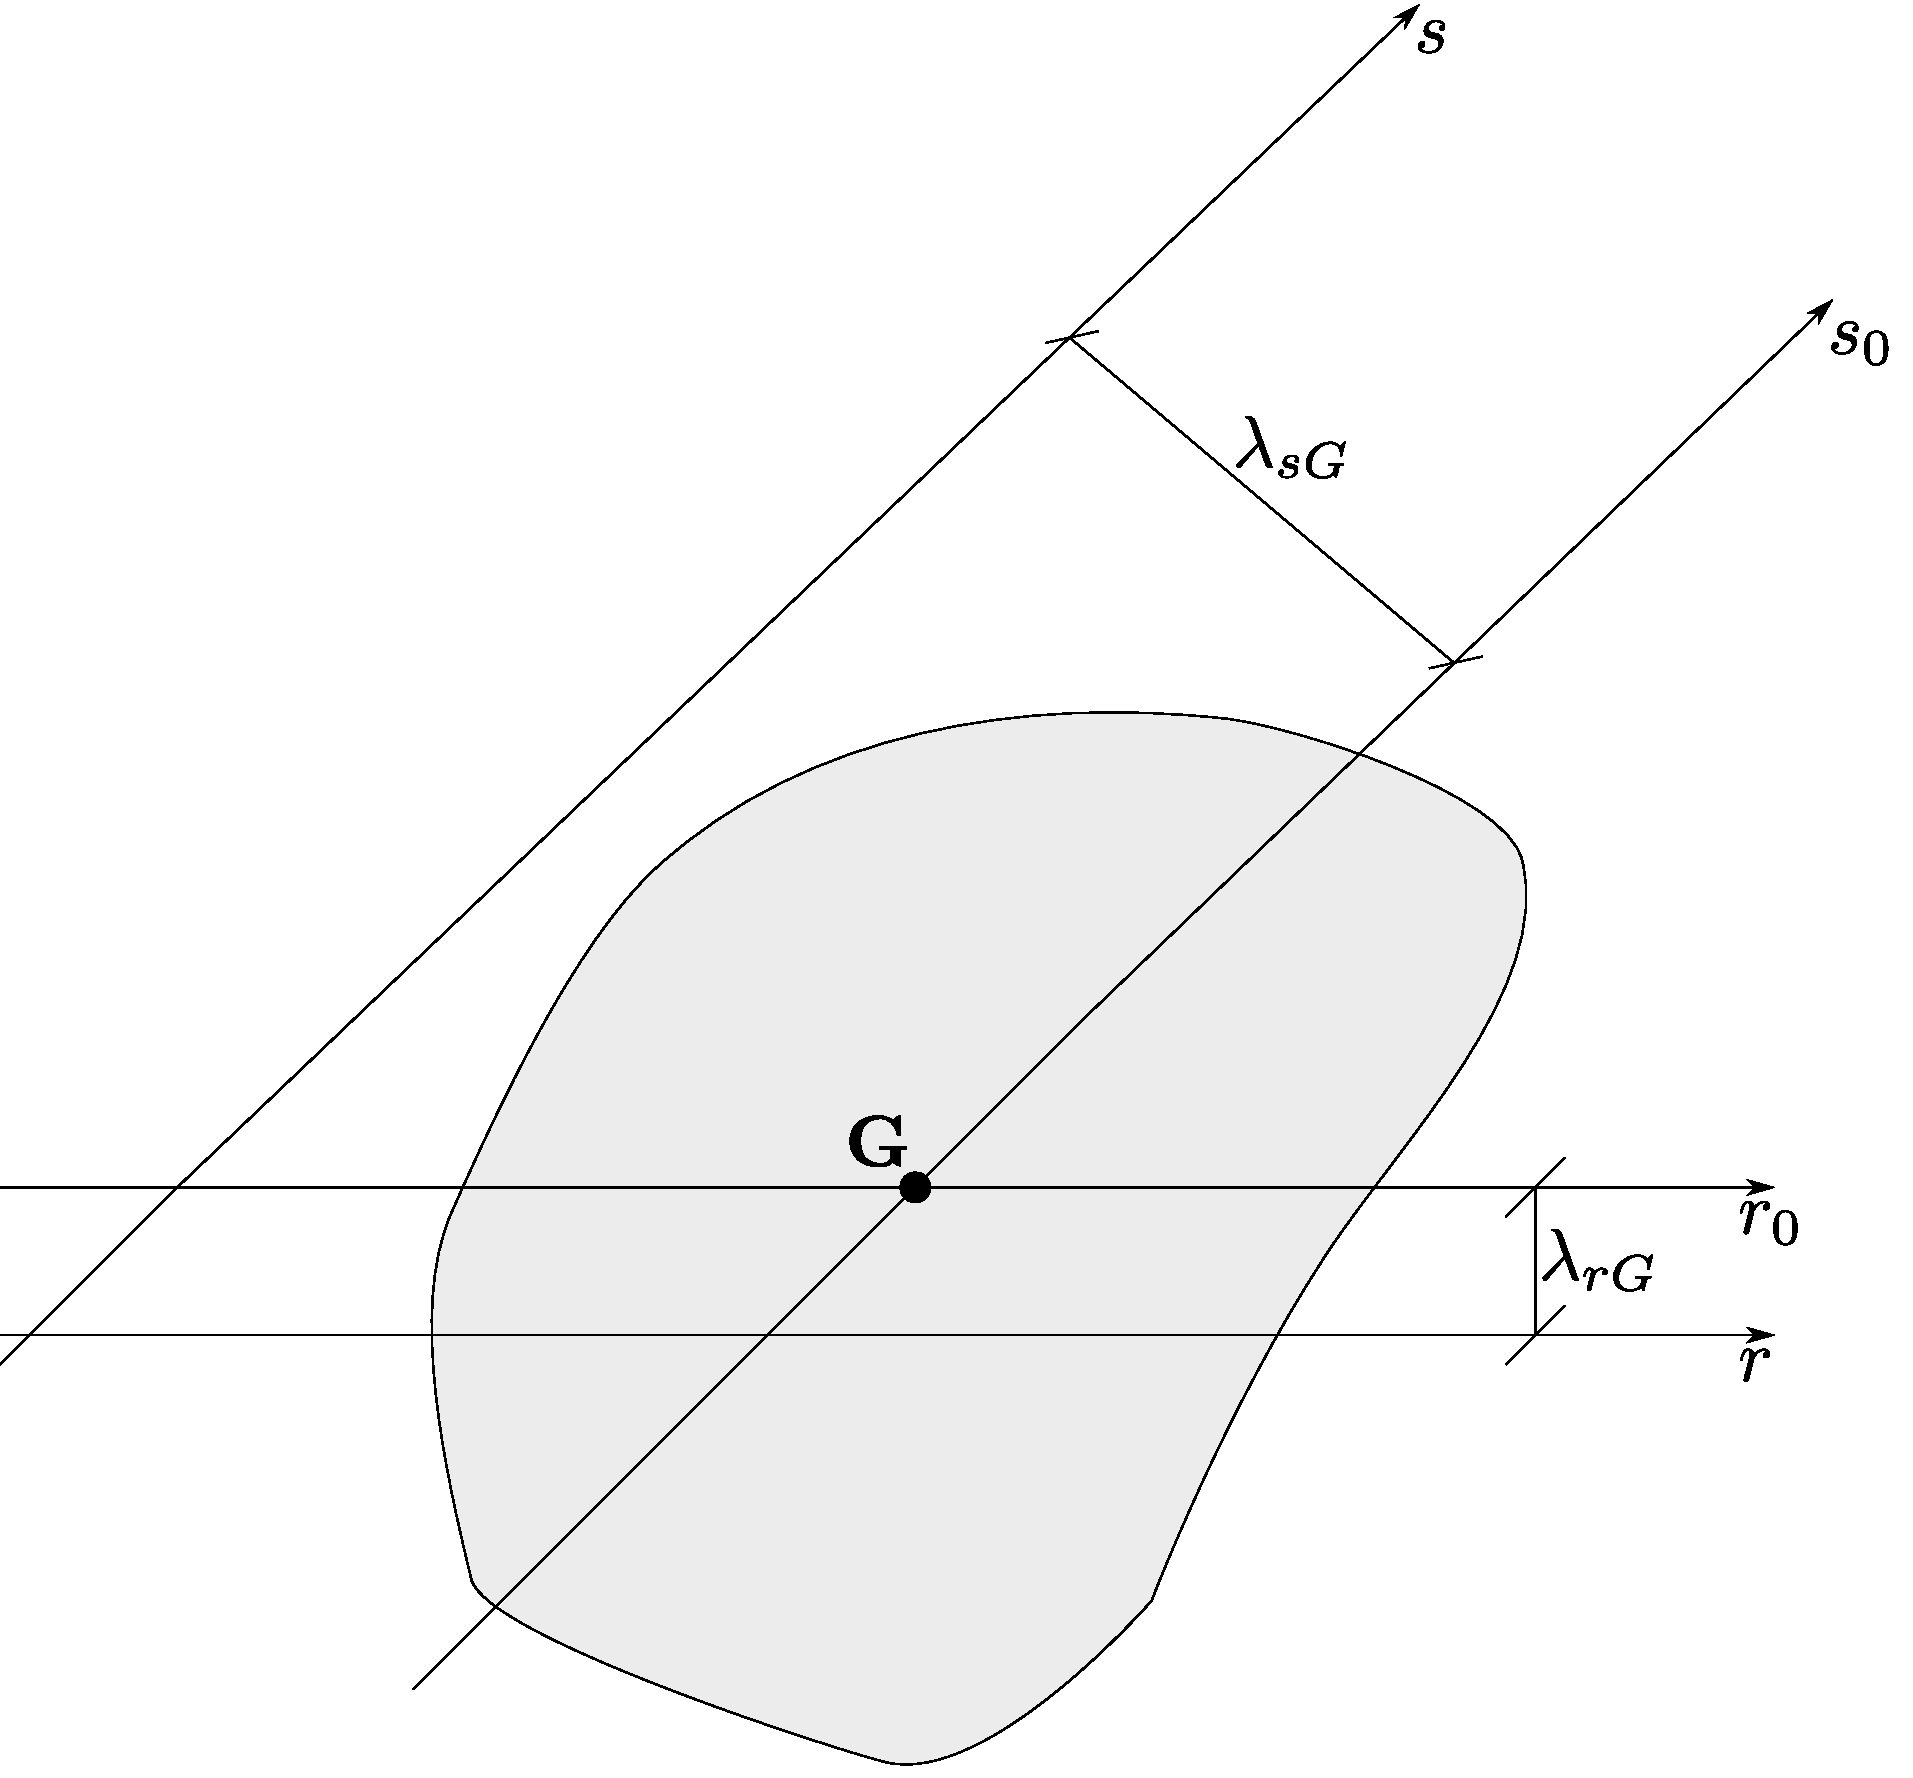
\includegraphics[width=0.73\textwidth]{Immagini/Parte_3/Figura3_5/Figura3_5.pdf}
\caption{}
\label{figura3-5}
\end{figure}
%--------------------------------------------------------------------------------------------------------------------------------------------------------------
\noindent Con riferimento alla figura~\ref{figura3-5}, si potrebbe dimostrare che 
%-------------------------------------------------------------------------------------------------------------------------------------------------------------
\begin{equation} \label{equazione3-4}
\boxed{I_{rs}=I_{r_{0}s_{0}}+A\lambda_{rG}\lambda_{sG}} \tag{3.4}
\end{equation}
%------------------------------------------------------------------------------------------------------------------------------------------------------------
Il termine $A\lambda_{rG}\lambda_{sG}$ è detto termine di trasporto; in esso $\lambda_{rG}$ e $\lambda_{sG}$ sono le distanze (con segno) del baricentro delle rette $r$ ed $s$; quindi $I_{rs}$ può essere maggiore o minore di zero. 
%--------------------------------------------------------------------------------------------------------------------------------------------------------------

\noindent Alla base della~\eqref{equazione3-4} è facile convincersi della seguente proposizione
%--------------------------------------------------------------------------------------------------------------------------------------------------------------
\begin{equation*}
\boxed{\textup{Se una retta passa per}\,\mathbf{G}\,\textup{e l'altra trasla, il momento centrifugo non varia}}
\end{equation*}
%--------------------------------------------------------------------------------------------------------------------------------------------------------------
Con riferimento alla~\ref{figura3-5}, la suddetta proposizione si traduce nei termini seguenti 
%--------------------------------------------------------------------------------------------------------------------------------------------------------------
\begin{align*}
I_{r_{0}s} &= I_{r_{0}s_{0}}, \quad \forall\,s\,\parallelsum\,s_{0} \\
I_{rs_{0}} &= I_{r_{0}s_{0}}, \quad \forall\,r\,\parallelsum\,r_{0}
\end{align*}
%--------------------------------------------------------------------------------------------------------------------------------------------------------------
Rispetto agli assi cartesiano il teorema del trasporto del momento centrifugo assume, ovviamente, la forma 
%-------------------------------------------------------------------------------------------------------------------------------------------------------------
\begin{equation} \label{equazione3-5}
\boxed{I_{xy}=I_{x_{0}y_{0}}+A\lambda_{x_{G}}\lambda_{y_{G}}} \tag{3.5}
\end{equation}
%------------------------------------------------------------------------------------------------------------------------------------------------------------
\section{Momenti centrifughi di un triangolo rettangolo}
%--------------------------------------------------------------------------------------------------------------------------------------------------------------
\renewcommand{\thefigure}{3~-~6}
\begin{figure}[ht]
\centering
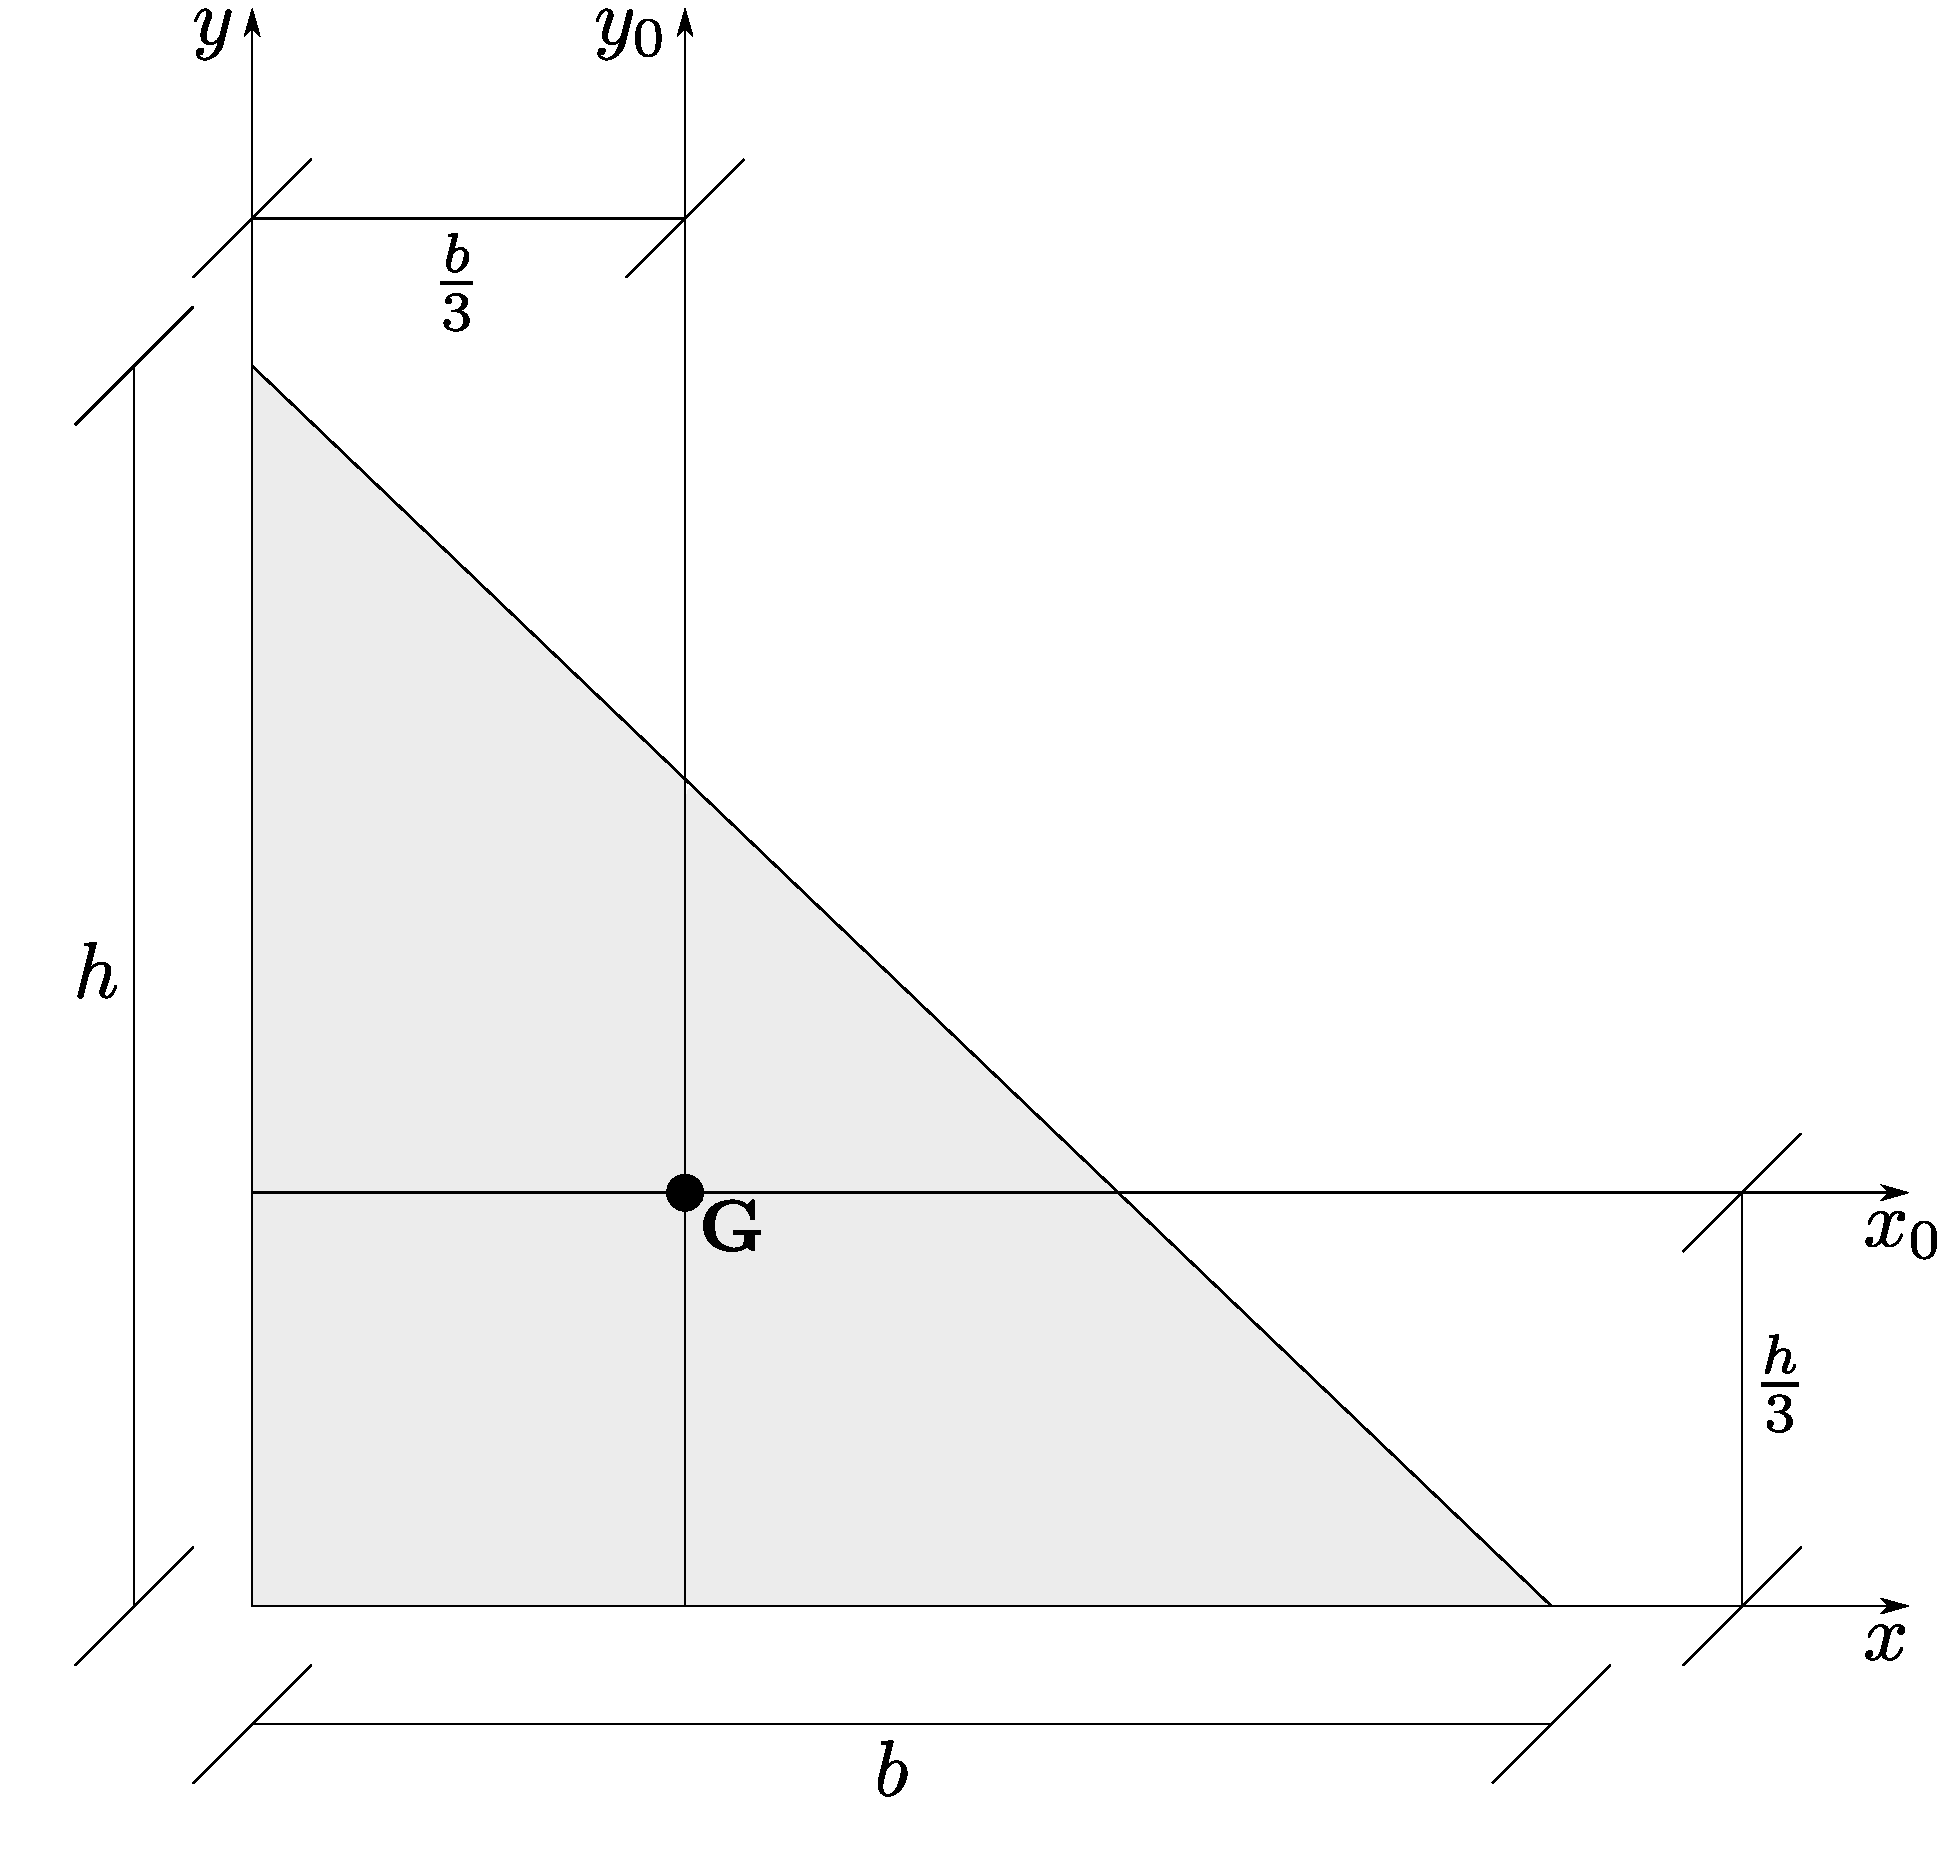
\includegraphics[width=0.62\textwidth]{Immagini/Parte_3/Figura3_6/Figura3_6.pdf}
\caption{}
\label{figura3-6}
\end{figure}
%--------------------------------------------------------------------------------------------------------------------------------------------------------------
\noindent Con riferimento alla figura~\ref{figura3-6}, ci proponiamo di calcolare prima $I_{xy}$ e poi, utilizzando il teorema del trasporto, $I_{x_{0}y_{0}}$. Cominciamo ad osservare che il lato $AB$ ha equazione
%--------------------------------------------------------------------------------------------------------------------------------------------------------------
\begin{equation*}
y = h - \frac{h}{b}x
\end{equation*}
%--------------------------------------------------------------------------------------------------------------------------------------------------------------
Dunque
%--------------------------------------------------------------------------------------------------------------------------------------------------------------
\begin{equation*}
I_{xy} = \int\int_A xydA = \int_{0}^{b}xdx\int_{0}^{h-\frac{h}{b}x}\!\!\!\!ydy = \int_{0}^{b}x\Biggl[\frac{1}{2}y^2\Biggr]_{0}^{b-\frac{h}{b}x}\!\!\!\!\!\!\!\!\!\!\!\!dx
\end{equation*}
%--------------------------------------------------------------------------------------------------------------------------------------------------------------
Ancora
%--------------------------------------------------------------------------------------------------------------------------------------------------------------
\begin{equation*}
I_{xy} = \frac{1}{2}\int_{0}^{b}x\biggl(h-\frac{h}{b}x\biggr)^{2}dx = \frac{h^{2}}{2}\int_{0}^{b}x\biggl(1+\frac{x^{2}}{b^{2}}-\frac{2}{b}x\biggr)dx = \frac{h^{2}}{2}\Biggl[\frac{x^{2}}{2}+\frac{x^4}{4b^{2}}-\frac{2}{3}\frac{x^{3}}{b}\Biggr]_{0}^{b}
\end{equation*}
%--------------------------------------------------------------------------------------------------------------------------------------------------------------
A conti fatti
%--------------------------------------------------------------------------------------------------------------------------------------------------------------
\begin{equation} \label{equazione3-6}
I_{xy} = \frac{b^{2}h^{2}}{24} \tag{3.6}
\end{equation}
%--------------------------------------------------------------------------------------------------------------------------------------------------------------
Applicando la~\eqref{equazione3-5}
%--------------------------------------------------------------------------------------------------------------------------------------------------------------
\begin{equation*}
I_{x_{0}y_{0}} = I_{xy} - Ax_{G}y_{G} = \frac{b^{2}h^{2}}{24}-\frac{1}{2}\frac{b^2}{3}\frac{h^2}{3}
\end{equation*}
%--------------------------------------------------------------------------------------------------------------------------------------------------------------
A conti fatti
%-------------------------------------------------------------------------------------------------------------------------------------------------------------
\begin{equation} \label{equazione3-7}
\boxed{I_{x_{0}y_{0}}=-\frac{b^{2}h^{2}}{72}} \tag{3.7}
\end{equation}
%--------------------------------------------------------------------------------------------------------------------------------------------------------------
\renewcommand{\thefigure}{3~-~7}
\begin{figure}[ht]
\centering
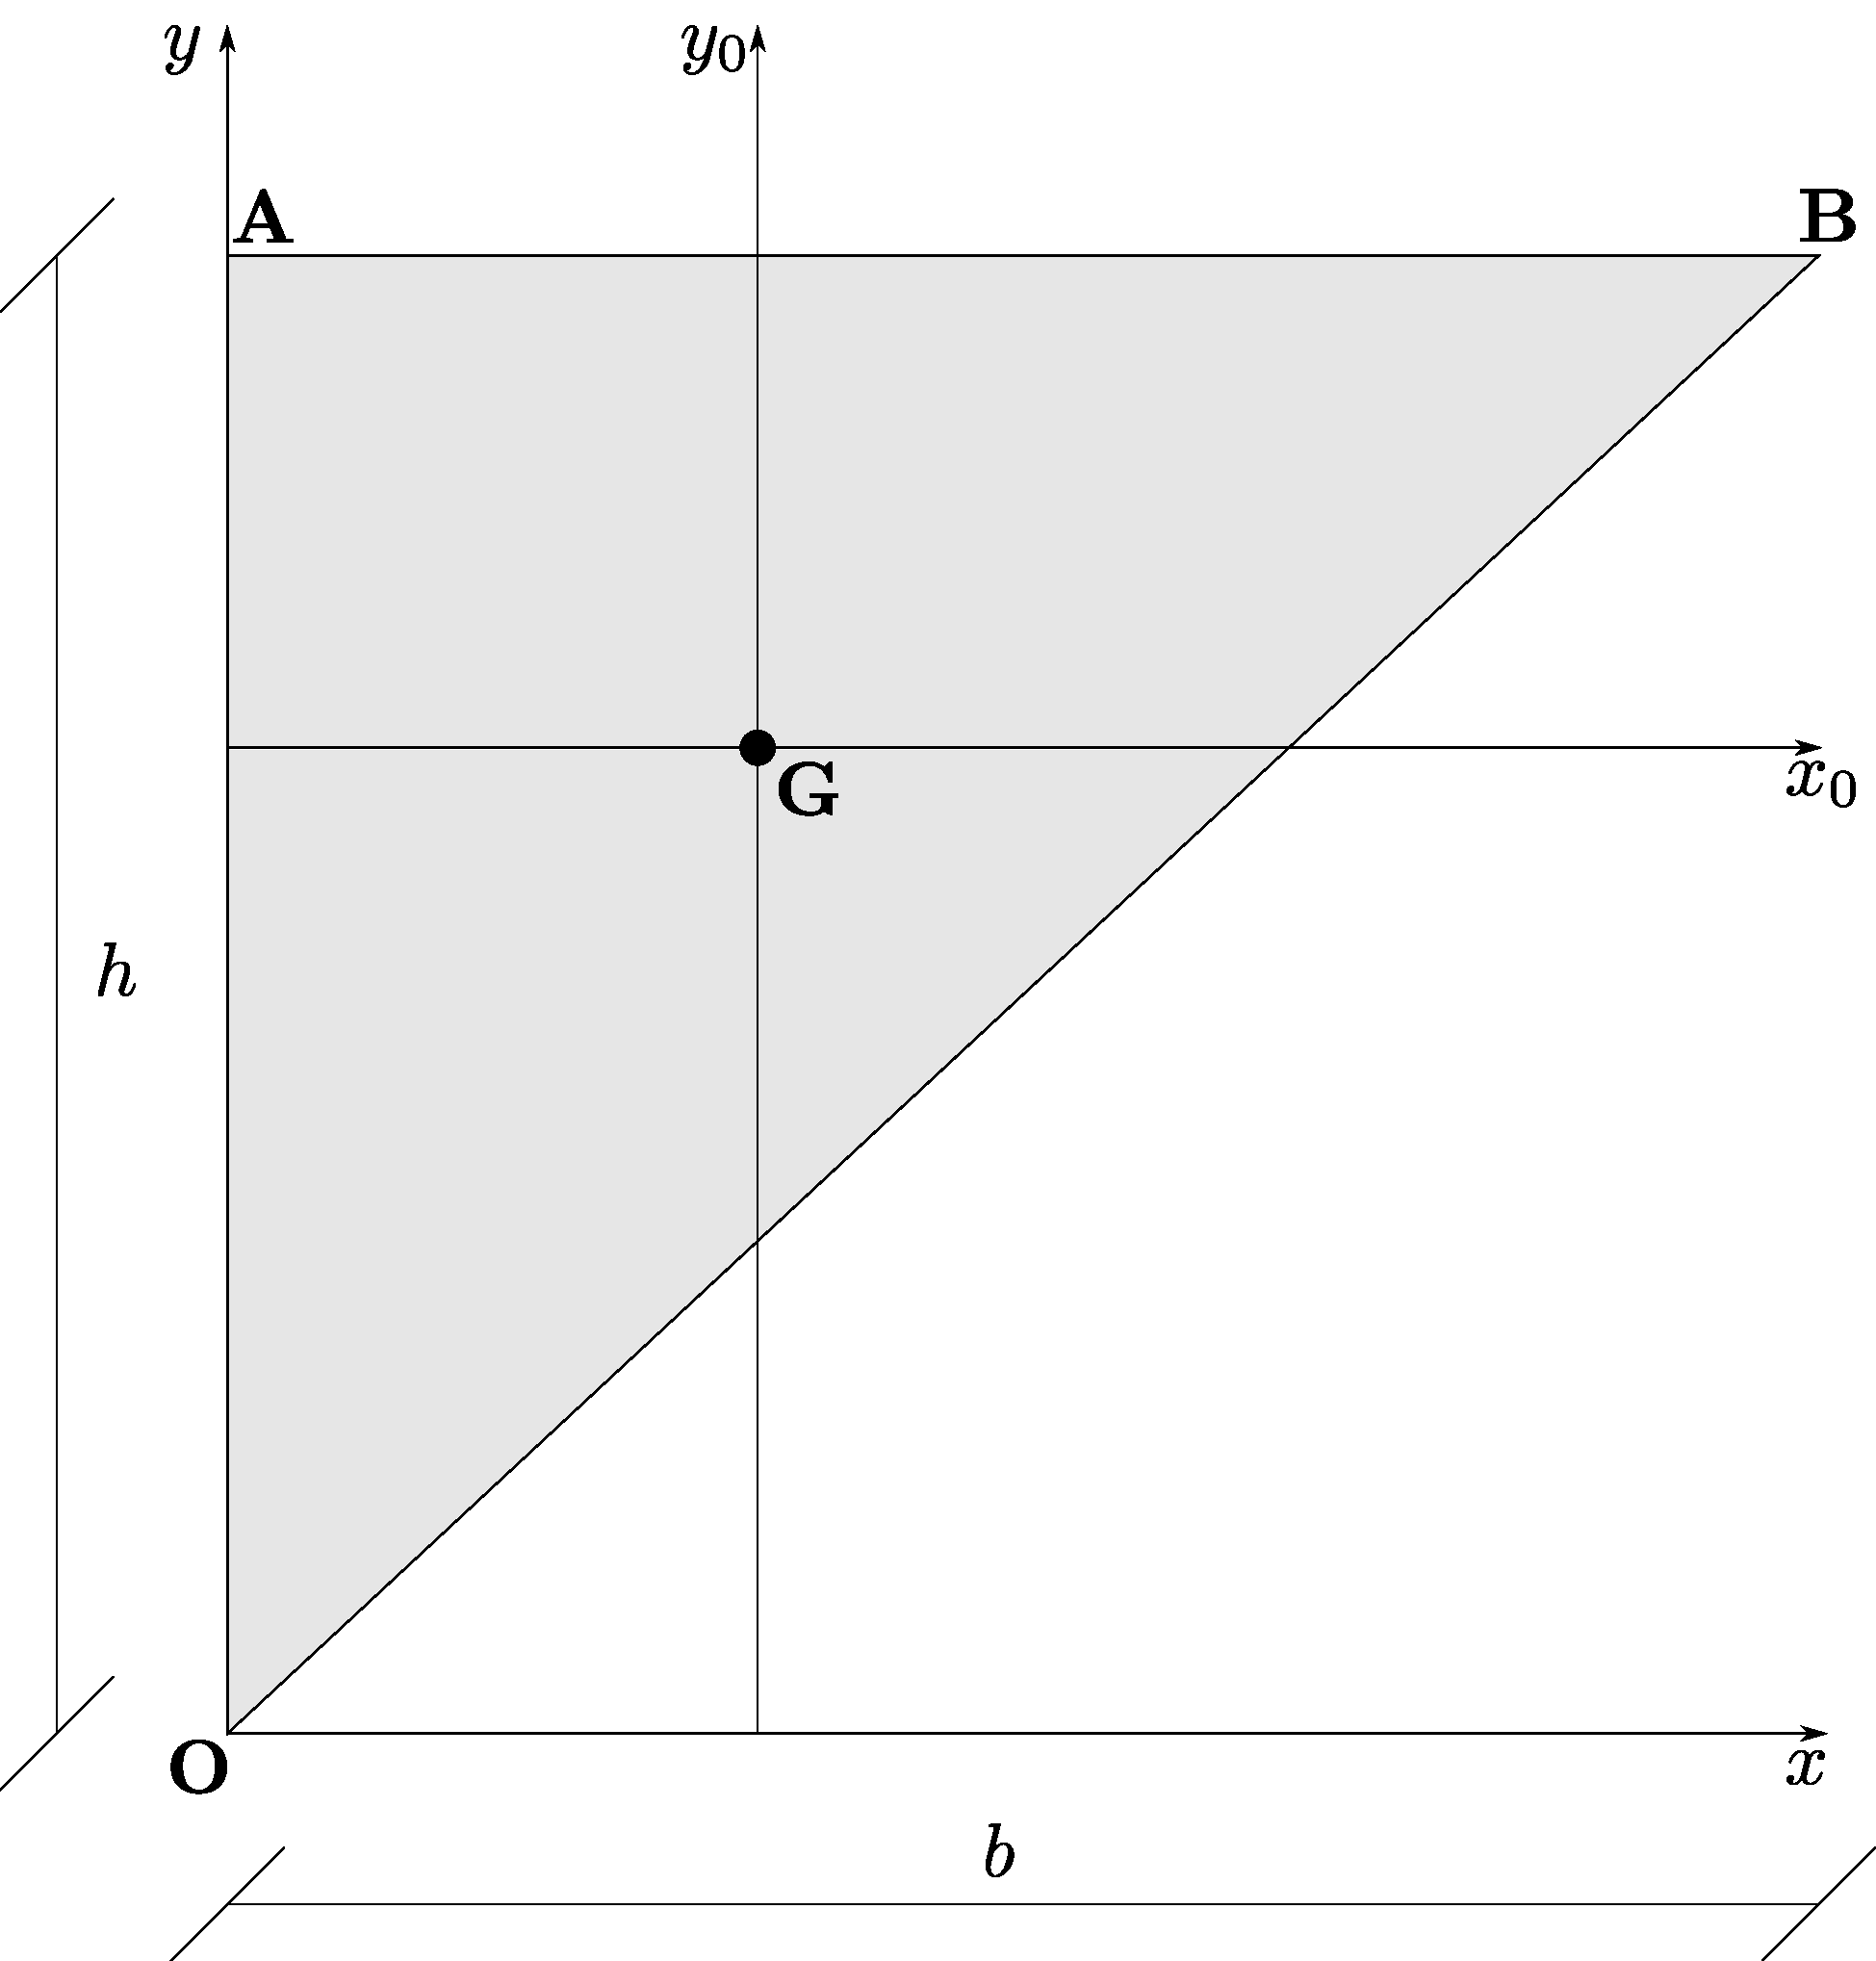
\includegraphics[width=0.45\textwidth]{Immagini/Parte_3/Figura3_7/Figura3_7.pdf}
\caption{}
\label{figura3-7}
\end{figure}
%--------------------------------------------------------------------------------------------------------------------------------------------------------------
Ed ora calcoleremo $I_{xy}$ e poi $I_{x_{0}y_{0}}$ per il triangolo rettangolo di figura~\ref{figura3-7}. Il lato $OB$ ha equazione
%--------------------------------------------------------------------------------------------------------------------------------------------------------------
\begin{equation*}
y = \frac{h}{b}x
\end{equation*}
%--------------------------------------------------------------------------------------------------------------------------------------------------------------
Dunque 
%--------------------------------------------------------------------------------------------------------------------------------------------------------------
\begin{equation*}
I_{xy} = \int\int_A xydA = \int_{0}^{b}xdx\int_{\frac{h}{b}x}^{b}ydy = \int_{0}^{b}x\biggl[\frac{1}{2}y^2\biggr]_{\frac{h}{b}x}^{b}\!\!\!\!\!\!dx = \frac{h^2}{2}\Biggl[\frac{x^2}{2}-\frac{x^4}{4b^2}\Biggr]_{0}^{b}
\end{equation*}
%--------------------------------------------------------------------------------------------------------------------------------------------------------------
A conti fatti
%--------------------------------------------------------------------------------------------------------------------------------------------------------------
\begin{equation} \label{equazione3-8}
\boxed{I_{xy}=\frac{h^{2}b^{2}}{8}}\tag{3.8}
\end{equation}
%--------------------------------------------------------------------------------------------------------------------------------------------------------------
Ed ora possiamo calcolare $I_{x_{0}y_{0}}$ applicando il teorema del trasporto
%--------------------------------------------------------------------------------------------------------------------------------------------------------------
\begin{equation*}
I_{x_{0}y_{0}} = I_{xy} - Ax_{G}y_{G} = \frac{h^{2}b^{2}}{8}-\frac{b^2}{3}\frac{h^2}{3}
\end{equation*}
%--------------------------------------------------------------------------------------------------------------------------------------------------------------
\clearpage
\section{Esercizi}
%--------------------------------------------------------------------------------------------------------------------------------------------------------------
\paragraph{Esercizi 3.1}
Calcolare $I_{xy}$ per il profilato riportato in figura.
\renewcommand{\thefigure}{3.1~-~1}
\begin{figure}[ht]
\centering
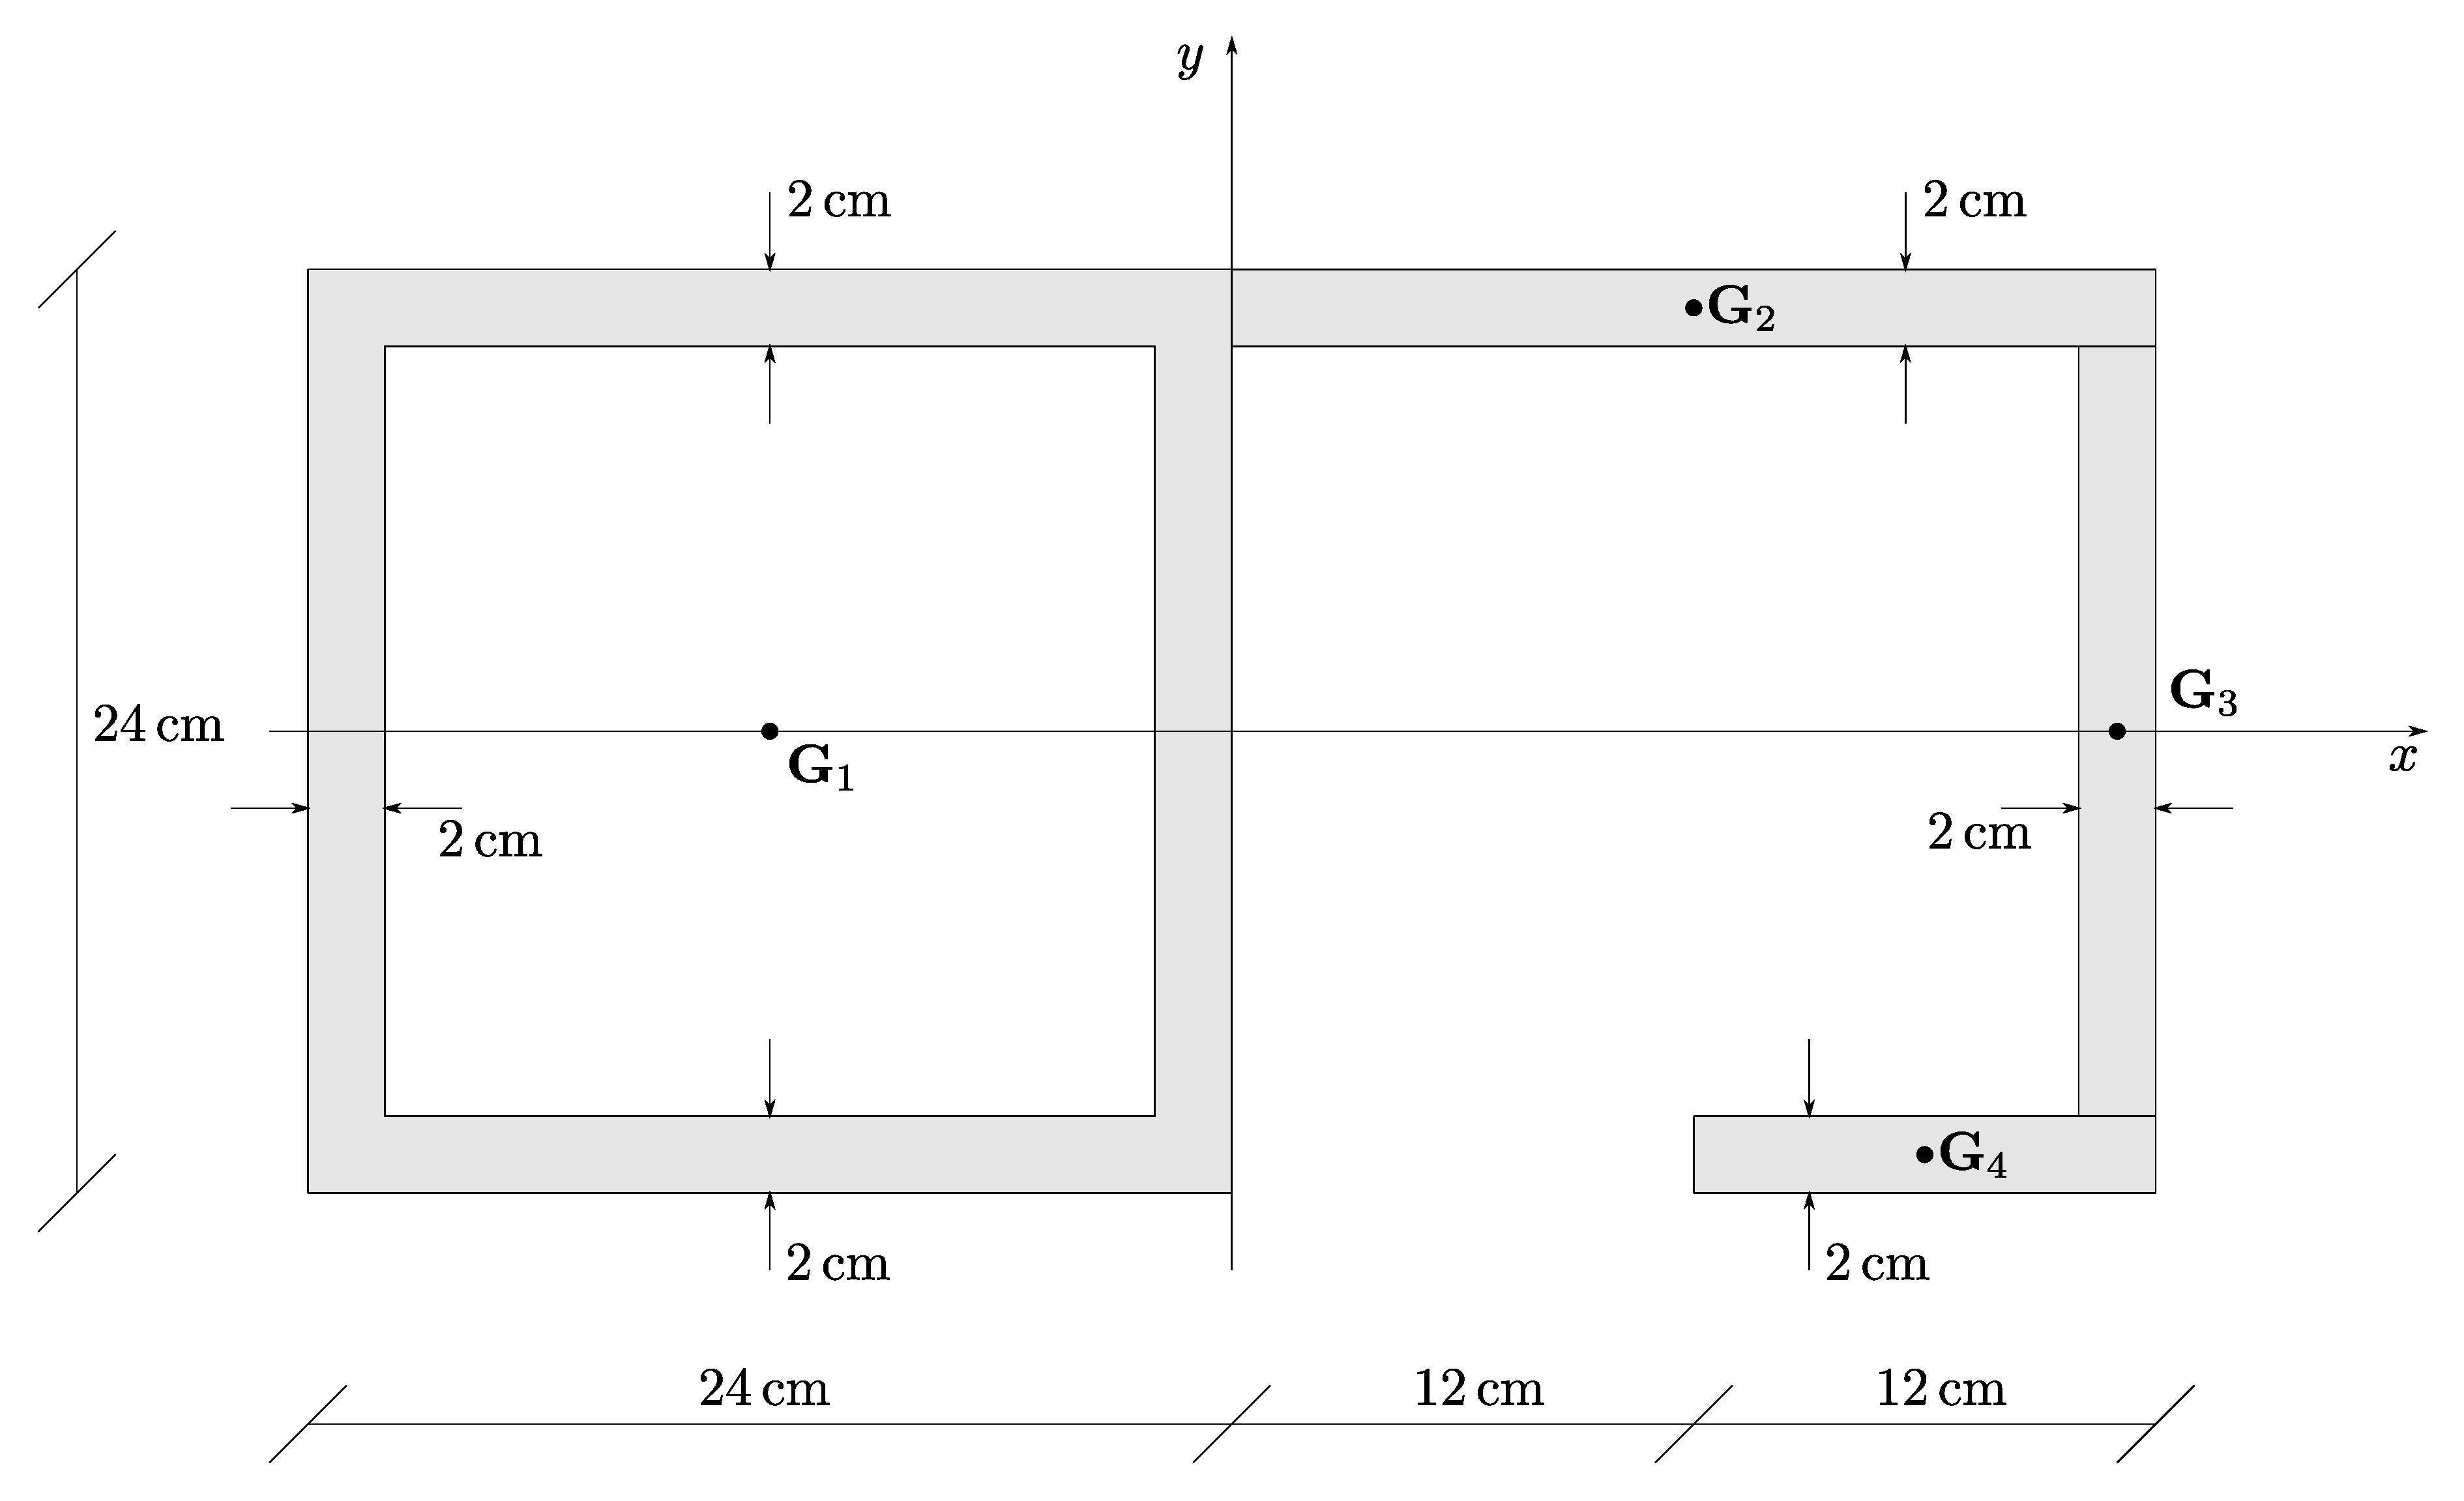
\includegraphics[width=\textwidth]{Immagini/Parte_3/Esercizio3_1/Esercizio3_1_1.pdf}
\caption{}
\label{Esercizio3_1}
\end{figure}
%--------------------------------------------------------------------------------------------------------------------------------------------------------------

\noindent Il profilato consiste di una parte \emph{chiusa}, il cui baricentro si è indicato con $\mathbf{G}_1$, e di tre rettangoli, i cui baricentri si sono indicati con $\mathbf{G}_2$, $\mathbf{G}_3$ e $\mathbf{G}_4$. 
%--------------------------------------------------------------------------------------------------------------------------------------------------------------
\begin{align*}
A_1 &= 24\times 24 -20\times 20 = 176\,\textup{cm}^2 \\ 
A_2 &= 24\times 2 = 48\,\textup{cm}^2 \\ 
A_3 &= 20\times 2 = 40\,\textup{cm}^2 \\ 
A_4 &= 12\times 2 = 24\,\textup{cm}^2
\end{align*}
%--------------------------------------------------------------------------------------------------------------------------------------------------------------
Le coordinate dei baricentri nel sistema di riferimento assunto sono
%--------------------------------------------------------------------------------------------------------------------------------------------------------------
\begin{align*}
&\mathbf{G}_1(-12, 0) \\
&\mathbf{G}_2(12, 11) \\
&\mathbf{G}_3(23, 0) \\
&\mathbf{G}_4(18, -11) 
\end{align*}
%--------------------------------------------------------------------------------------------------------------------------------------------------------------
Per ognuna delle quattro parti costituenti il nostro profilato, risulta nullo il momento centrifugo rispetto ai due assi passanti per i rispettivi baricentri e paralleli ad $x$ ed $y$; pertanto, applicando il teorema del trasporto
%-------------------------------------------------------------------------------------------------------------------------------------------------------------
\begin{align*}
I_{1xy} &= I_{1x_{0}y_{0}}+A_{1}x_{G_{1}}y_{G_{1}} = 0+0 = 0 \\ 
I_{2xy} &= I_{2x_{0}y_{0}}+A_{2}x_{G_{2}}y_{G_{2}} = 0+48\times 12\times 11 = 6336\,\textup{cm}^4 \\ 
I_{3xy} &= I_{3x_{0}y_{0}}+A_{3}x_{G_{3}}y_{G_{3}} = 0+0 = 0 \\ 
I_{4xy} &= I_{4x_{0}y_{0}}+A_{4}x_{G_{4}}y_{G_{4}} = 0+24\times 18\times (-11) = -4752\,\textup{cm}^4
\end{align*}
%--------------------------------------------------------------------------------------------------------------------------------------------------------------
In definitiva, essendo il momento centrifugo una grandezza additiva come l'area, il momento statico ed il momento di inerzia
%--------------------------------------------------------------------------------------------------------------------------------------------------------------
\begin{equation*}
I_{xy} = 6336-4752 = 1584\,\textup{cm}^4
\end{equation*}
%--------------------------------------------------------------------------------------------------------------------------------------------------------------
\clearpage
\paragraph{Esercizio 3.2}
Calcolare il momento centrifugo $I_{xy}$ per il settore di corona circolare di spessore molto sottile già considerato nell'Esercizio $1.7$.
%--------------------------------------------------------------------------------------------------------------------------------------------------------------
\newline 

\noindent Al solito 
%--------------------------------------------------------------------------------------------------------------------------------------------------------------
\begin{align*}
I_{xy} &= \int\int_A xydA = \int\int_A (r\cos\varphi)(r\sin\varphi)rdrd\varphi = \int_{R_i}^{R_e}r^{3}dr\int_{\alpha}^{\beta} \sin\varphi\cos\varphi d\varphi \\
          &= \frac{R_{e}^{4}-R_{i}^{4}}{4}\frac{1}{2}\bigl[\sin^{2}\varphi\bigr]_{\alpha}^{\beta}
\end{align*}
%--------------------------------------------------------------------------------------------------------------------------------------------------------------
In definitiva si ottiene 
%--------------------------------------------------------------------------------------------------------------------------------------------------------------
\begin{equation*}
\boxed{\textup{\textsc{Formula esatta}}} \longrightarrow \boxed{I_{xy} = \frac{R_{e}^{4}-R_{i}^{4}}{8}(\sin^{2}\beta-\sin^{2}\alpha)}
\end{equation*}
%--------------------------------------------------------------------------------------------------------------------------------------------------------------
Posto
%--------------------------------------------------------------------------------------------------------------------------------------------------------------
\begin{align*}
R_e &= r_m + \frac{\delta}{2} \\
R_i  &= r_m - \frac{\delta}{2}
\end{align*}
%--------------------------------------------------------------------------------------------------------------------------------------------------------------
si trova 
%--------------------------------------------------------------------------------------------------------------------------------------------------------------
\begin{equation*}
R_{e}^{4}-R_{i}^{4} = r_{m}\delta(4r_{m}^{2}+\delta^2) = r_{m}^{2}\delta\biggl(4+\frac{\delta^2}{r_{m}^{2}}\biggr)
\end{equation*}
%--------------------------------------------------------------------------------------------------------------------------------------------------------------
Trascurando il termine $\frac{\delta^2}{r_{m}^{2}}$ rispetto a $4$
%--------------------------------------------------------------------------------------------------------------------------------------------------------------
\begin{equation*}
R_{e}^{4}-R_{i}^{4} \equiv 4r_{m}^{3}\delta 
\end{equation*}
%--------------------------------------------------------------------------------------------------------------------------------------------------------------
e quindi
%--------------------------------------------------------------------------------------------------------------------------------------------------------------
\begin{equation*}
\boxed{\textup{\textsc{Formula approssimata}}} \longrightarrow \boxed{I_{xy} = \frac{1}{2}r_{m}^{3}\delta(\sin^{2}\beta-\sin^{2}\alpha)}
\end{equation*}
%--------------------------------------------------------------------------------------------------------------------------------------------------------------
L'errore insito nella formula approssimata, nel caso in cui $\frac{\delta}{r_{m}}=10$, è un po' minore dello $0.25\%$.
%--------------------------------------------------------------------------------------------------------------------------------------------------------------